\subsubsection{Abstract}
Digital television allows interactive content to accompany standard broadcasts. The development of bespoke interactive content is expensive. You are to design a system that will allow the non-technical producers of television programmes to build interactive content from a set of high-level building blocks.
In effect, you will create a modelling language (metamodel, rules and symbols), a tool supporting it, and a generator.

\subsubsection{Background}
Digital television is becoming increasingly popular in the UK. In addition to providing higher quality video and increased channel capacity, it allows interactive content to accompany standard broadcasts. Interactive applications have been used to enhance traditional broadcasts in many ways:

\begin{itemize}
	\item Viewers can play along with quizzes (Figure \ref{fig:MDDTIFFigure1}).
	\item Viewers can choose different camera angles during sporting events
	\item Viewers can take part in discussions and comment on events though message boards.
	\item Viewers can remind themselves of the important developments in a drama's plot (Figure \ref{fig:MDDTIFFigure2}).
\end{itemize}

\begin{figure}
	\centering
		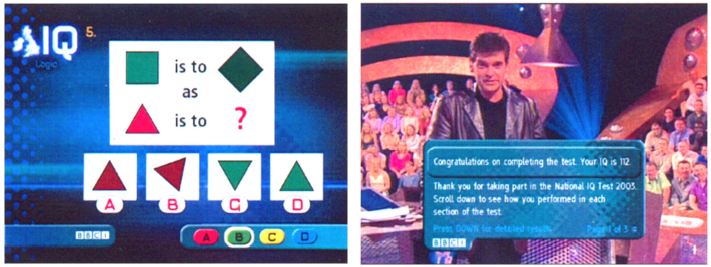
\includegraphics[width=1\textwidth]{images/MDDTIFFigure1.png}
	\caption{Playing along with Test the Nation}
	\label{fig:MDDTIFFigure1}
\end{figure}

\begin{figure}
	\centering
		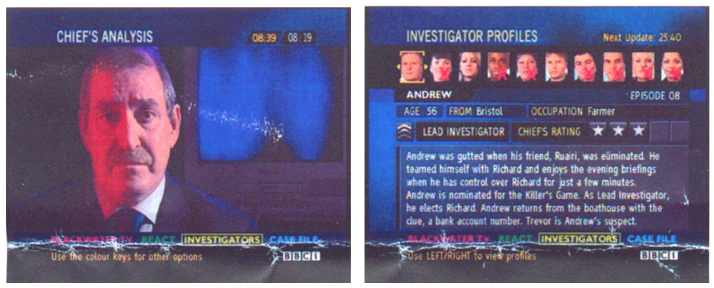
\includegraphics[width=1\textwidth]{images/MDDTIFFigure2.png}
	\caption{Viewing developments in The Murder Game}
	\label{fig:MDDTIFFigure2}
\end{figure}

\subsubsection{Problem}
Currently, each interactive application is bespoke. This greatly limits the number of programmes that can be accompanied by interactive content, as the applications are expensive to develop. The resulting UI is also different for different programmes, which is confusing to users. You are to design a system that will allow non-technical producers to build applications to accompany their programmes.

The application will sit on the right hand side of the screen (Figure \ref{fig:MDDTIFFigure3}), and display one of the following pieces of content:

\begin{itemize}
	\item A page of text, to be used for news stories, background information etc.
	\item A multiple choice vote, for example \emph{Man of the match} in a football match.
	\item A menu that allows the user to view items of content, including sub-menus.
\end{itemize}

The basic on-screen layout and navigational structure of the application has been defined by the user experience department, and producers are not able to change it.

\begin{figure}
	\centering
		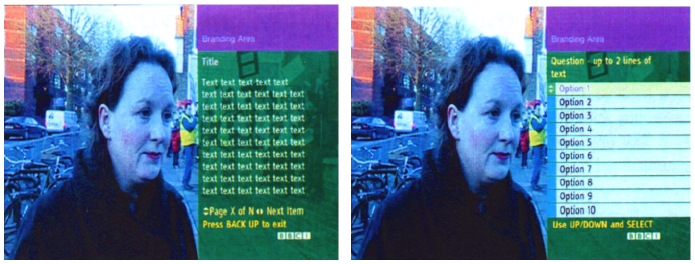
\includegraphics[width=1\textwidth]{images/MDDTIFFigure3.png}
	\caption{Different types of content}
	\label{fig:MDDTIFFigure3}
\end{figure}

\subsubsection{Use cases}
The following set of use cases emerged during discussions with the producers. They are ordered by their value to the producers, with the use case giving the most value first.

\paragraph{Case 1}
A producer would like to build an application for the soccer world cup finals, listing the teams and information about each, and allowing viewers to vote for the most likely winner.

\paragraph{Case 2}
As Case 1, but the teams should be listed by group (e.g. four teams in three groups). As the
teams are known before their division into groups by lots, it should be possible to define the
content for the teams first, and quickly add the structure of the groups, so that the application
can be running for users as soon as possible during the program that broadcasts the division
by lots.

\paragraph{Case 3}
A producer would like to use a page of text to provide analysis of the recent events in a rugby
match. A journalist with a laptop will need to change the text on the page throughout the
match. The user interface used by the journalist should not allow him to change the structure
of the whole application, only edit the text.

\paragraph{Case 4}
A producer has decided that the wording of a particular text page was better before the last
set of changes, and would like to revert it.

\subsubsection{Interactive application architecture}
Designing interactive applications requires relatively detailed knowledge of the standards for
each platform. For this reason, you should concentrate on the system used by producers to
define the application content, and its interfaces to black box components that build the
actual application. To define these interfaces, you will need some knowledge of the basic
architecture of interactive applications. The following crash-course should suffice.
Digital televisions contain a basic operating system, and a set of libraries providing functions
to display text and graphics, change the currently displayed video stream, etc. Applications
are designed and specified with a domain-specific modelling language (that you develop)
and delivered to digital televisions by inserting it as XML into the same broadcast stream that
contains the video and audio content. Once running, an application can be updated by
changing the XML in the broadcast stream. Applications can send reply messages to your
system, usually via a standard modem built into the television. Sending these reply messages
is very slow, and involves the viewer paying call charges. For these reasons, reply
messages can only be used for viewer initiated actions, such as responding to a vote.

\subsubsection{Code generation}
You should generate code like the following as plain text, rather than using any special
method for saving models as XML. This puts the various tools on an even footing, and
demonstrates the code generation facilities better for all kinds of code and other output files.
Handling white space and encodings is not vital, but the results should be machine and
human-readable.

\begin{lstlisting}[basicstyle=\ttfamily\footnotesize, flexiblecolumns=true, numbers=none, nolol=true, caption=Sample Generated XML, label=lst:MDDTIFXML, language=XML, tabsize=2]
<TVApp name=�World Cup 2010�>
	<Menu name=�World Cup�>
		<Vote name=�Who will win?�>
			<Choice name=�Estonia�/>
			<Choice name=�Lithuania�/>
		</Vote>
		<Text name=�World Cup trivia�>Trinidad &amp; 
			Tobago were the first ...</Text>
		<Menu name=�Teams�>
		�
		</Menu>
	</Menu>
</TVApp>
\end{lstlisting}
